\documentclass[a4paper, handout]{beamer}
\usepackage{graphicx}
\graphicspath{ {./images/} }

\begin{document}

\begin{frame}
	\frametitle{Overleven}
	\begin{figure}
		\centering
	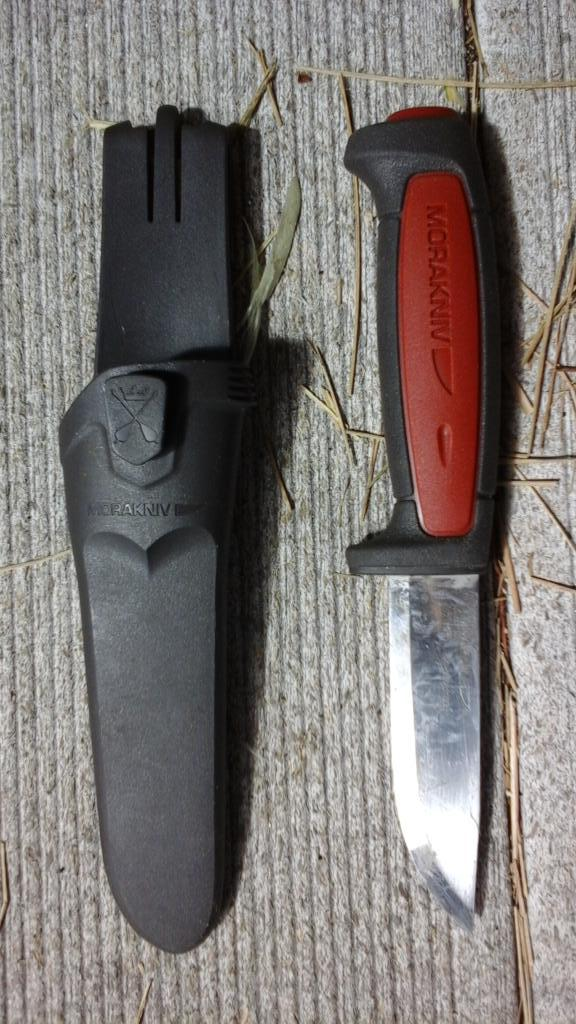
\includegraphics[scale=0.2]{mes}
\end{figure}

Wat is belangrijk om te overleven?
\end{frame}
\begin{frame}
	\frametitle{Hoe je kunt overleven}
	Om te kunnen overleven heb je nodig:
	\begin{enumerate}
		\item{Vuur}
		\item{Water}
		\item{Voedsel}
		\item{Beschutting}
	\end{enumerate}
\end{frame}

\begin{frame}
	\frametitle{Je hebt vuur nodig om}
	\begin{enumerate}
		\item{Water te zuiveren}
		\item{Warmte te geven}
		\item{Te koken}
		\item{Wilde dieren af te schrikken}
	\end{enumerate}
\end{frame}

\begin{frame}
	\frametitle{Vuur basis}
	Vuur krijg je alleen maar als de volgende dingen er zijn:
	\begin{enumerate}
		\item{Brandstof}
		\item{Zuurstof}
		\item{Hitte}
	\end{enumerate}
	Wij gaan verder kijken naar wrijvingsvuur.
\end{frame}

\begin{frame}
	\frametitle{Wrijvingsvuur}
	Wij gebruiken als basis	
	\begin{description}
		\item[Brandstof] pluizen, stro, twijgjes en groter hout
		\item[Zuurstof] 20 procent van de lucht is zuurstof
		\item[Hitte] wrijving!
	\end{description}
\end{frame}

\begin{frame}
	\frametitle{Vuurboog}
	Voor een vuurboog heb je nodig:
	
	\begin{description}
		\item[Snaar] stevig stuk touw van minimaal een meter
		\item[Boog] kromme stok van 50 tot 70 centimeter lang
		\item[Dop] een stuk steen met een holte om druk te leveren
		\item[Opvanger] stukje dun hout om het kooltje te vangen
		\item[Boor] een rechte tak van 15 tot 20 millimeter dik en tussen de 15 en 30 centimeter lang
		\item[Vuurbord] een plankje van 15 tot 25 millimeter dik, minimaal twee keer de breedte van de dikte van de boor. En 20 centimeter lang.
	\end{description}
\end{frame}

\begin{frame}
	\frametitle{Houtsoorten}
	Voor een vuurbord en boor gebruik je het liefst dezelfde soort hout.

	De beste soorten zijn zachte houtsoorten zoals:
	\begin{enumerate}
		\item{Naaldbomen}
		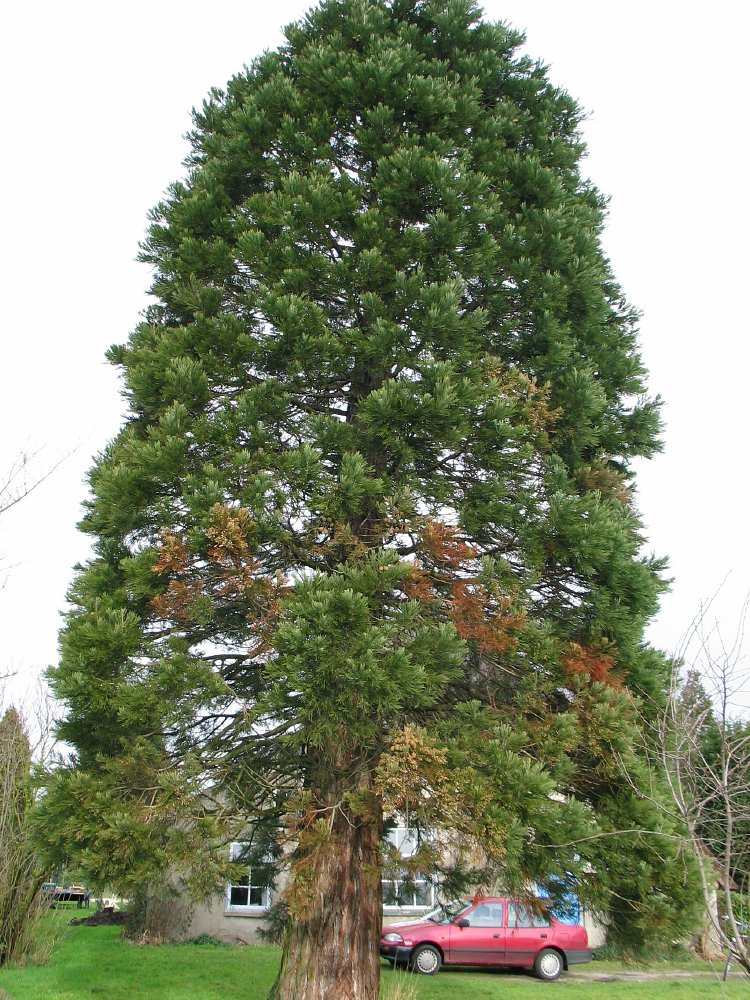
\includegraphics[scale=0.07]{naaldboom}
		\item{Wilg}
		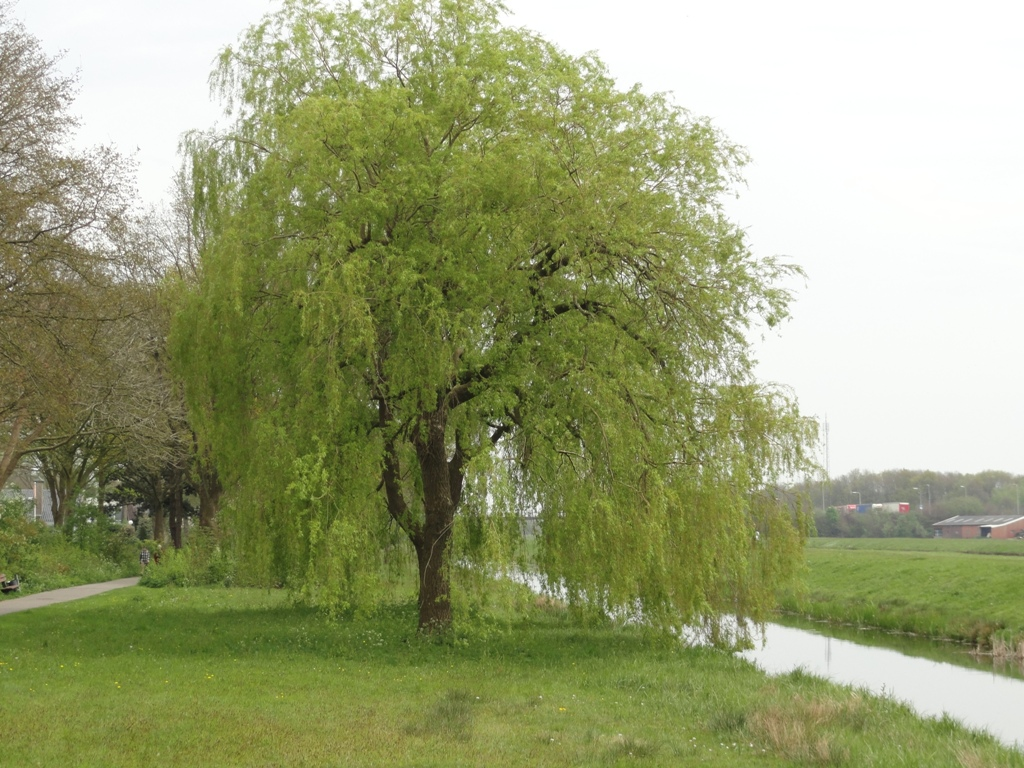
\includegraphics[scale=0.08]{wilg}
		\item{Populier}
		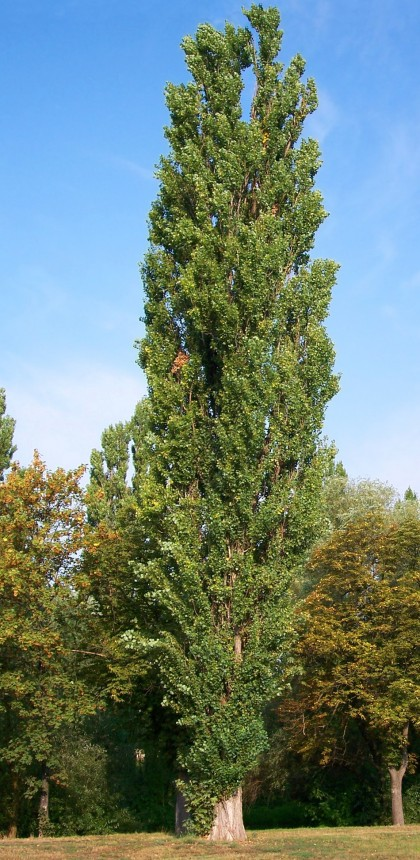
\includegraphics[scale=0.08]{populier}
	\end{enumerate}
	
\end{frame}

\begin{frame}
	\frametitle{Hout voor boor en bord}
	Gebruik geen levend hout, want dat is veel te nat.

		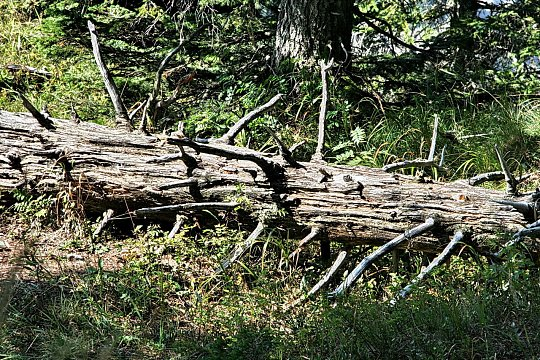
\includegraphics[width=0.80\textwidth]{dode-boom}

	Haal zijtakken van een liggende dode boom, die niet de grond raken.
\end{frame}

\begin{frame}
	\frametitle{Boor maken}
	Een vuurboor heeft de vorm een dik potlood met gum. Met de botte kant gaan we boren in het vuurbord, want we willen veel wrijving.

	\begin{tabular}{ c c }
		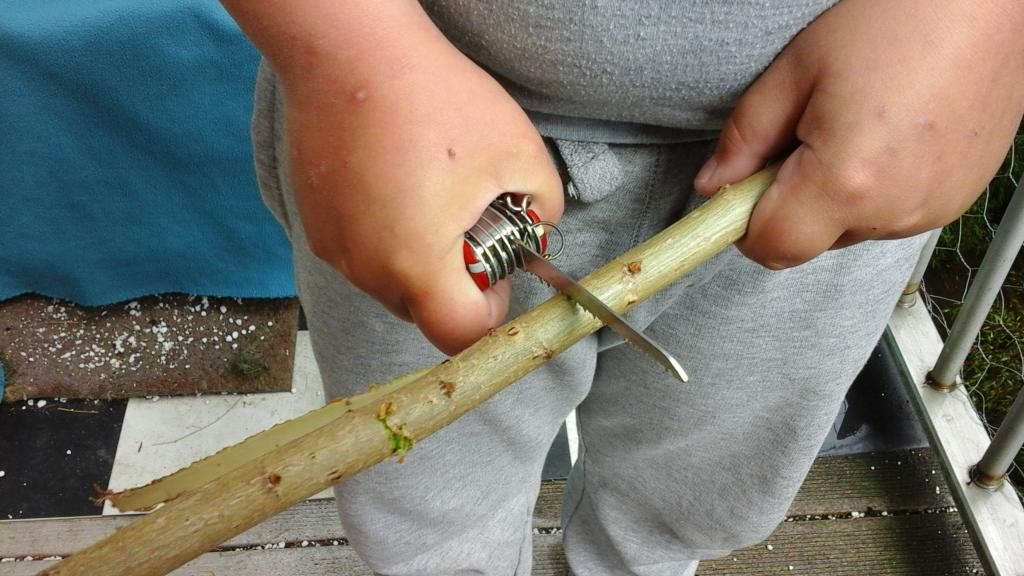
\includegraphics[scale=0.14]{boor-maken-1}
		&
		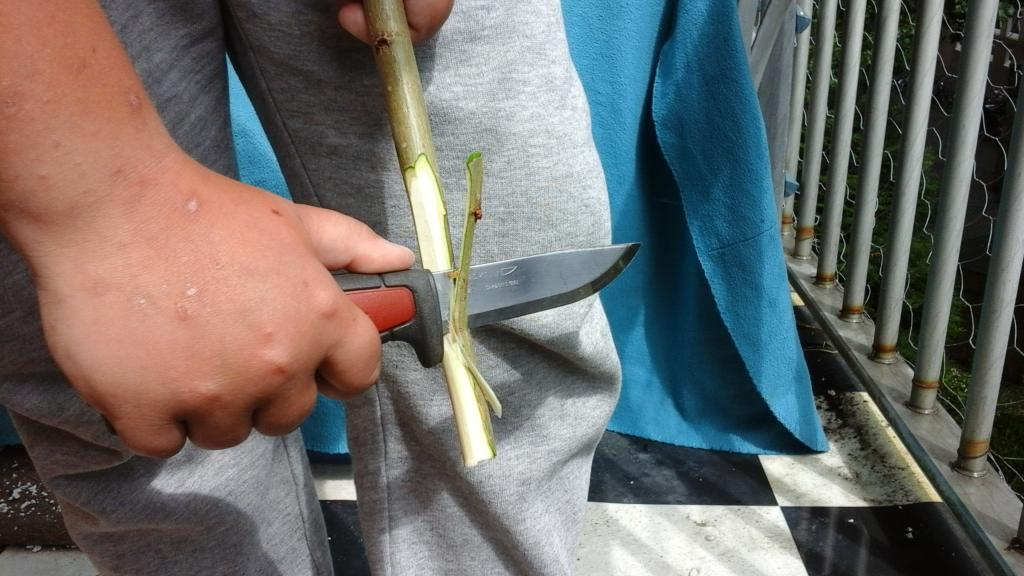
\includegraphics[scale=0.14]{boor-maken-2}
		\\
		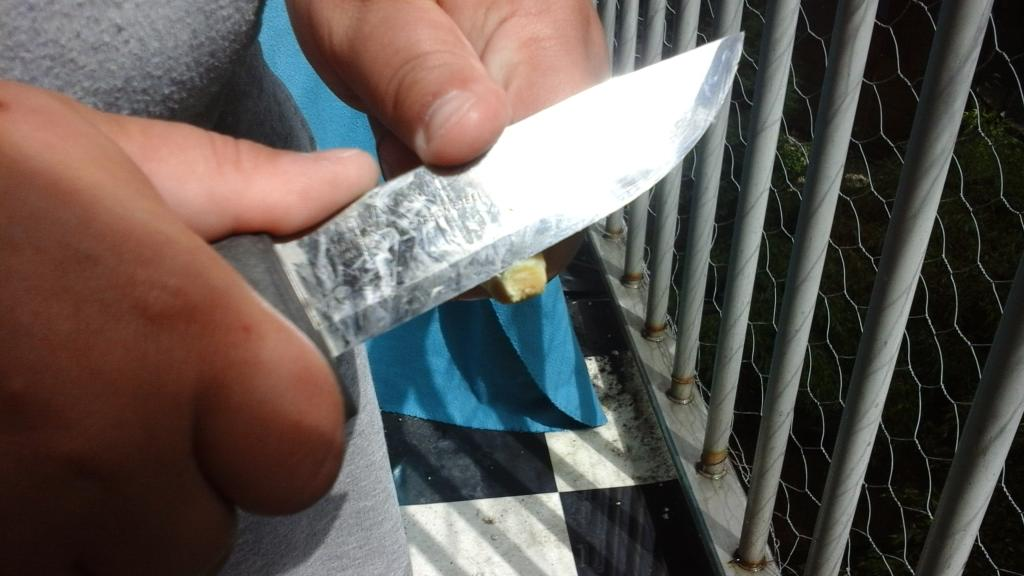
\includegraphics[scale=0.14]{boor-maken-3}
		&
		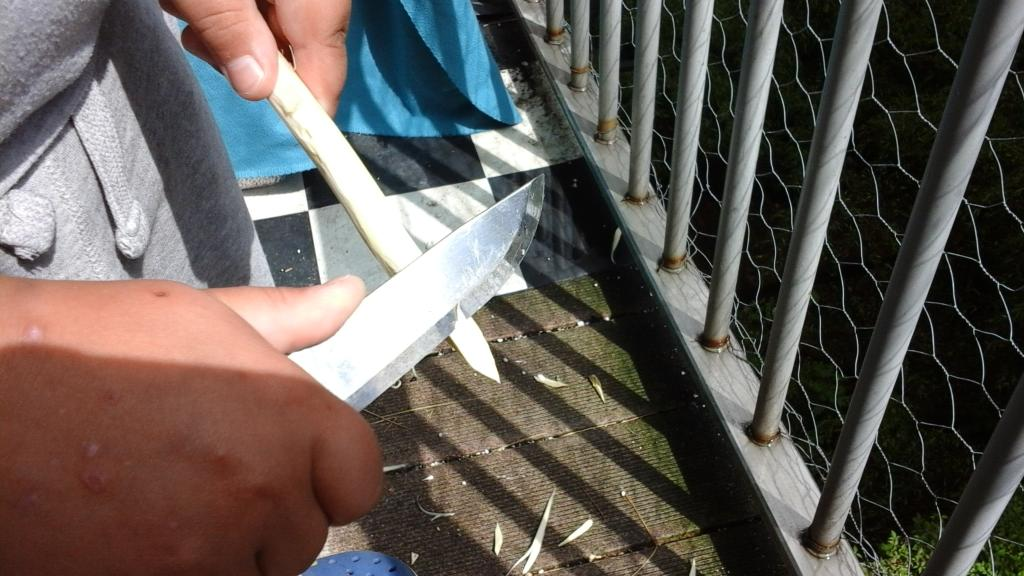
\includegraphics[scale=0.14]{boor-maken-4}
		\\
	\end{tabular}
\end{frame}

\begin{frame}
	\frametitle{Vuurboog maken}
	Je kunt aan de uiteindes van de boog een gleufje zagen waarin je de snaar vastmaakt.

	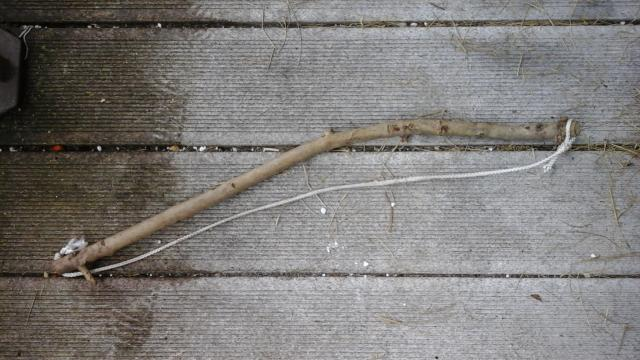
\includegraphics[scale=0.4]{vuurboog}
\end{frame}

\begin{frame}
	\frametitle{Indraaien van boor op het bord}
	\begin{tabular}{ c c }
		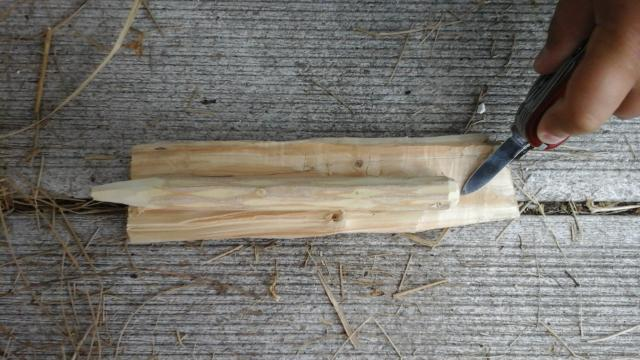
\includegraphics[scale=0.16]{indraaien-1}
		&
		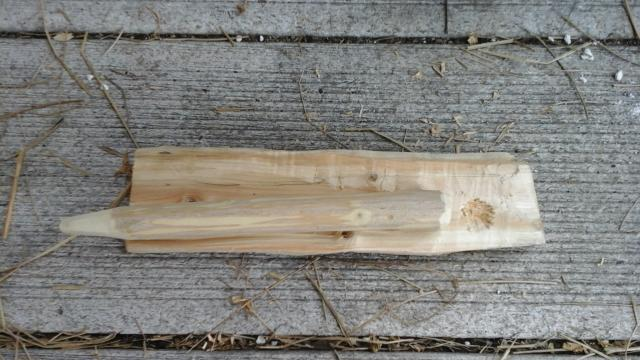
\includegraphics[scale=0.16]{indraaien-2}
		\\
		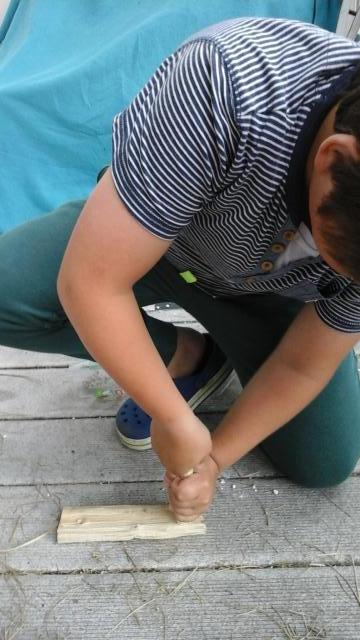
\includegraphics[scale=0.16]{indraaien-3}
		&
		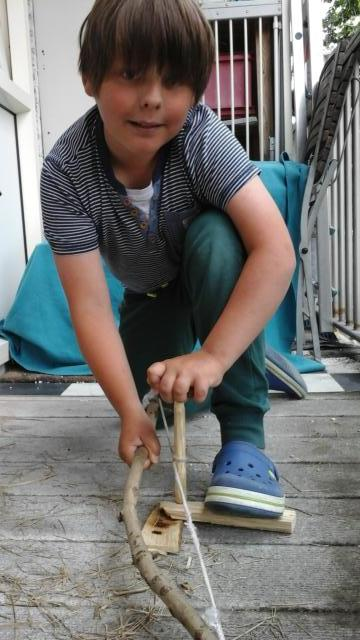
\includegraphics[scale=0.16]{indraaien-4}
		\\
		\multicolumn{2}{c}{ 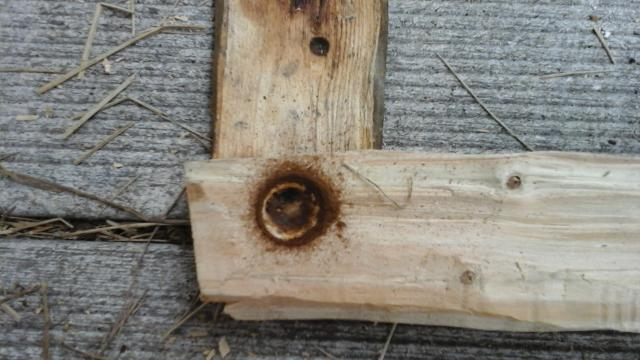
\includegraphics[scale=0.16]{indraaien-5}}
	\end{tabular}
\end{frame}

\begin{frame}
	\frametitle{Vogelnestje maken}
	\begin{tabular}{ c c }
		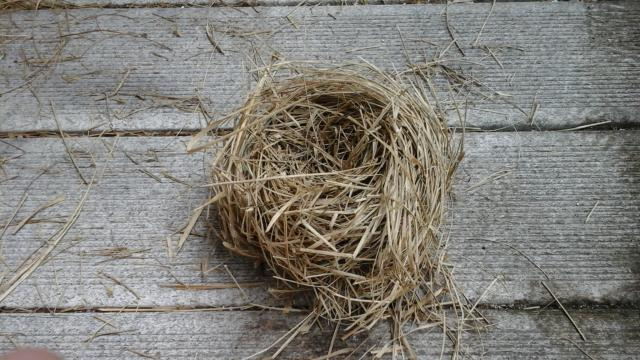
\includegraphics[scale=0.3]{nestje-1}
		&
		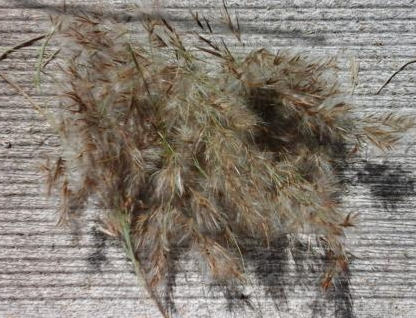
\includegraphics[scale=0.3]{nestje-2}
		\\
		\multicolumn{2}{c}{ 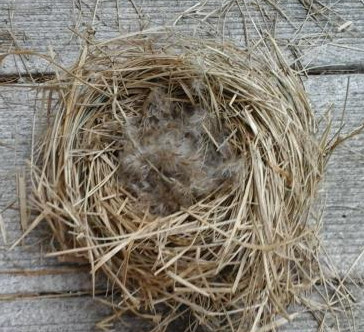
\includegraphics[scale=0.3]{nestje-3}}
		\\
	\end{tabular}
\end{frame}

\begin{frame}
	\frametitle{Inkeping voor het stof maken}
	\begin{tabular}{ c c }
		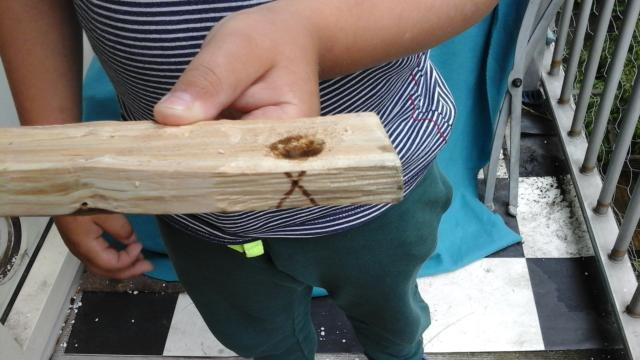
\includegraphics[scale=0.15]{inkeping-1}
		&
		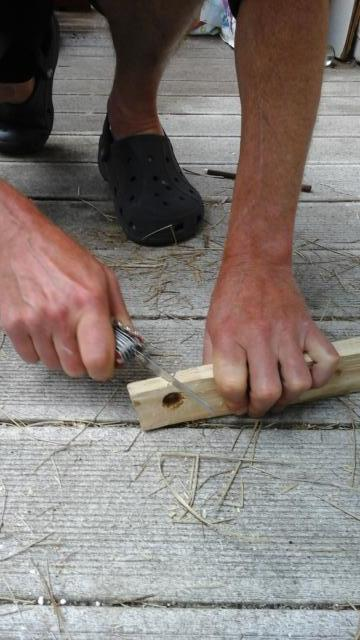
\includegraphics[scale=0.20]{inkeping-2}
		\\
		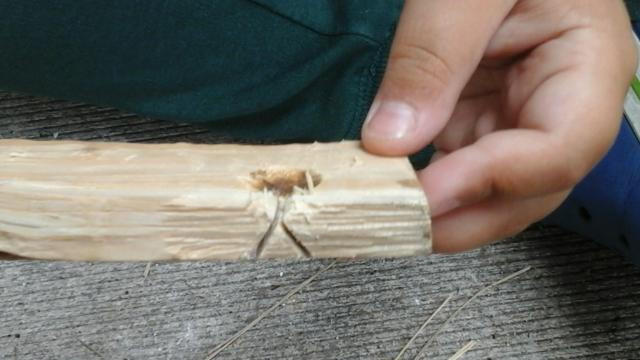
\includegraphics[scale=0.15]{inkeping-3}
		&
		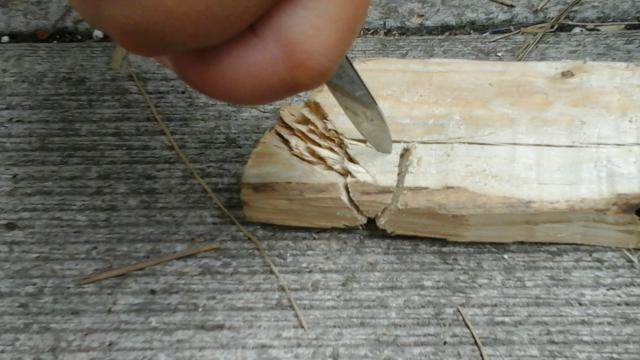
\includegraphics[scale=0.15]{inkeping-4}
		\\
		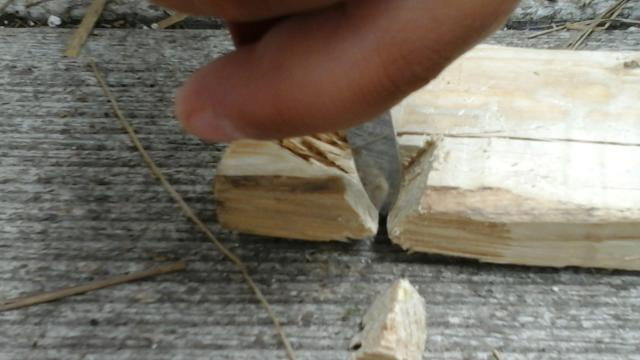
\includegraphics[scale=0.15]{inkeping-5}
		&
		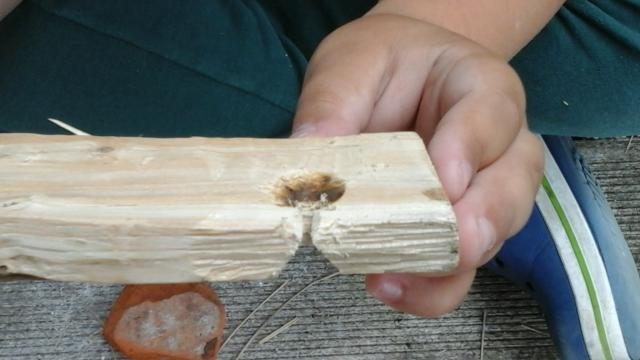
\includegraphics[scale=0.15]{inkeping-6}
		\\
	\end{tabular}
\end{frame}

\begin{frame}
	\frametitle{Boren voor kooltje}
	\begin{tabular}{ c c }
		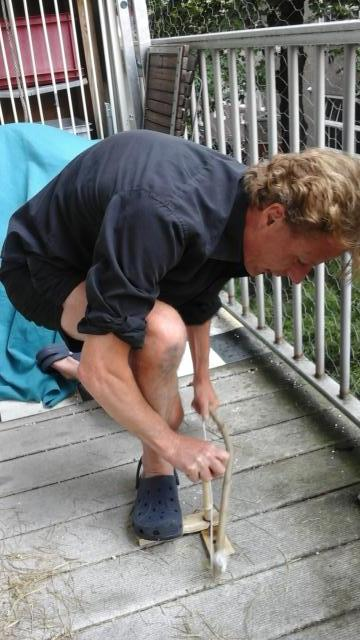
\includegraphics[scale=0.22]{boren-1}
		&
		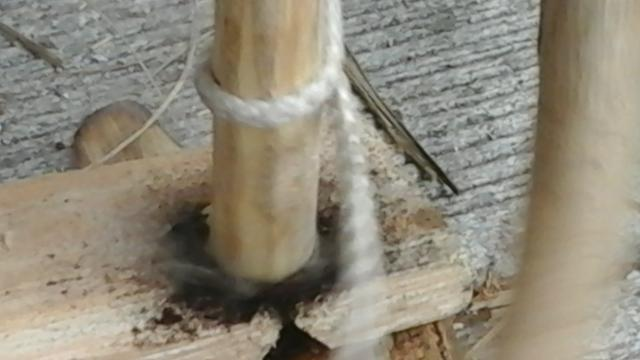
\includegraphics[scale=0.32]{boren-2}
		\\
		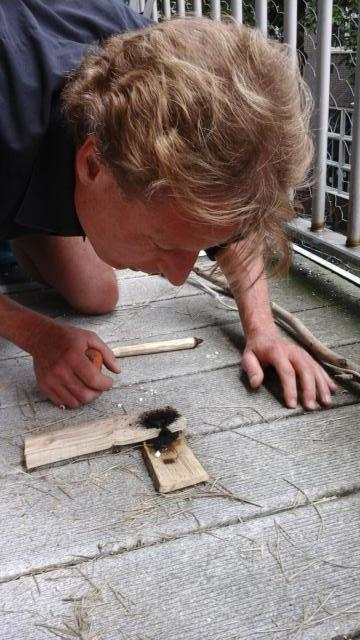
\includegraphics[scale=0.22]{boren-3}
		&
		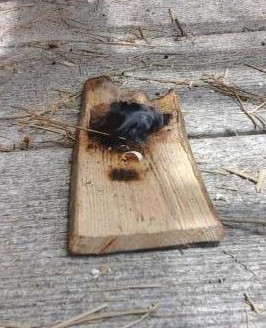
\includegraphics[scale=0.35]{boren-4}
		\\
	\end{tabular}
\end{frame}

\begin{frame}
	\frametitle{Kooltje in het vogelnestje doen en aanblazen}
	\begin{tabular}{ c c }
		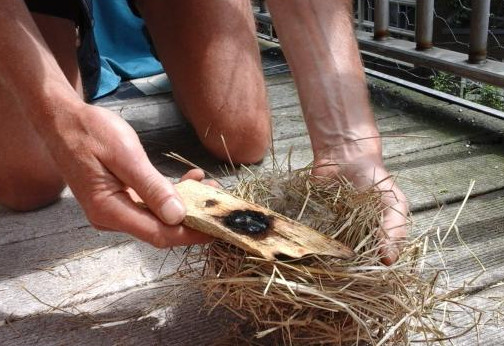
\includegraphics[height=0.40\textheight]{blazen-1}
		&
		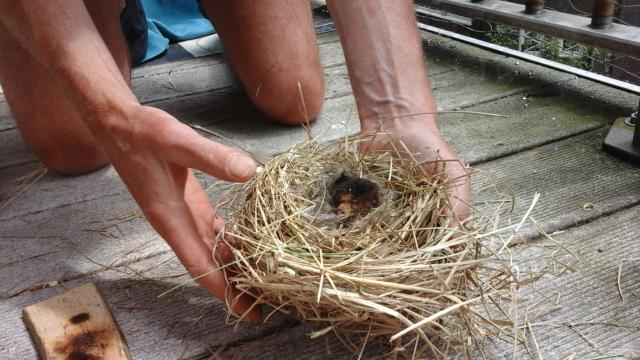
\includegraphics[height=0.40\textheight]{blazen-2}
		\\
		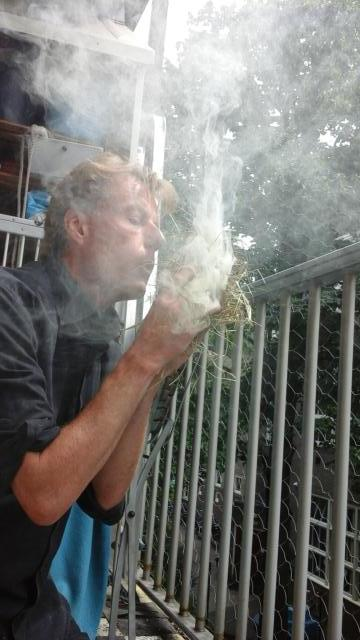
\includegraphics[height=0.40\textheight]{blazen-3}
		&
		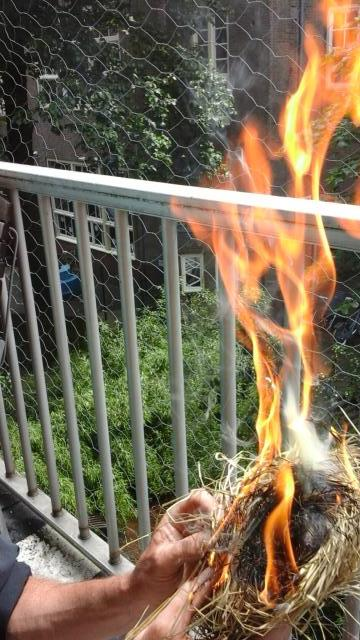
\includegraphics[height=0.40\textheight]{blazen-4}
		\\
	\end{tabular}
\end{frame}

\begin{frame}
	\frametitle{Demonstratie}
	Demonstratie van vuurboog
\end{frame}

\begin{frame}
	\frametitle{Quizvraag 1}
	Welke drie dingen heeft een vuur nodig?
\end{frame}

\begin{frame}
	\frametitle{Antwoord 1}
	Welke drie dingen heeft een vuur nodig?
	\begin{enumerate}
		\item{Brandstof}
		\item{Zuurstof}
		\item{Hitte}
	\end{enumerate}
\end{frame}
\begin{frame}
	\frametitle{Quizvraag 2}
	Noem zoveel mogelijke onderdelen van het vuur maken met de boog.
\end{frame}

\begin{frame}
	\frametitle{Antwoord 2}
	Noem zoveel mogelijke onderdelen van het vuur maken met de boog.
	\begin{enumerate}
		\item{Snaar}
		\item{Boog}
		\item{Dop}
		\item{Opvanger}
		\item{Boor}
		\item{Vuurbord}
	\end{enumerate}
\end{frame}

\begin{frame}
	\frametitle{Quizvraag 3}
	Wat zijn de vier belangrijkste dingen om te overleven?
\end{frame}

\begin{frame}
	\frametitle{Antwoord 3}
	Wat zijn de vier belangrijkste dingen om te overleven?
	\begin{enumerate}
		\item{Vuur}
		\item{Water}
		\item{Voedsel}
		\item{Beschutting}
	\end{enumerate}
\end{frame}

\begin{frame}
	\frametitle{Vragen}
	Zijn er nog vragen?
\end{frame}

\begin{frame}
	\frametitle{Tips en tops}
	Heeft er iemand een tip of top?
\end{frame}

\begin{frame}
	\frametitle{Einde}
	Bedankt voor jullie aandacht.	
\end{frame}
\end{document}

